% This is an example of using latex for a paper/report of specified
% size/layout. It's useful if you want to provide a PDF that looks
% like it was made in a normal word processor.

% While writing, don't stop for errors
\nonstopmode

% Use the article doc class, with an 11 pt basic font size
\documentclass[12pt, a4paper]{article}

% Makes the main font Nimbus Roman, a Times New Roman lookalike:
%\usepackage{mathptmx}% http://ctan.org/pkg/mathptmx
% OR use this for proper Times New Roman (from msttcorefonts package
% on Ubuntu). Use xelatex instead of pdflatex to compile:
\usepackage{fontspec}
\usepackage{xltxtra}
\usepackage{xunicode}
\defaultfontfeatures{Scale=MatchLowercase,Mapping=tex-text}
\setmainfont{Times New Roman}
% Set margins
\usepackage[margin=2.5cm]{geometry}
% Multilingual support
\usepackage[english]{babel}
% Nice mathematics
\usepackage{amsmath}
% Control over maketitle
\usepackage{titling}
% Section styling
\usepackage{titlesec}
% Syntax highlighted code listing
\usepackage{listings}
% Ability to use colour in text
\usepackage[usenames]{color}
% Colours for code
%\usepackage{xcolor}
\definecolor{codegreen}{rgb}{0,0.6,0}
\definecolor{codered}{rgb}{0.95,0.0,0.0}
\definecolor{codegray}{rgb}{0.5,0.5,0.5}
\definecolor{codepurple}{rgb}{0.58,0,0.82}
\definecolor{backcolour}{rgb}{1,1,1}
\lstdefinestyle{mystyle}{
    backgroundcolor=\color{backcolour},
    commentstyle=\color{codered},
    keywordstyle=\color{codepurple},
    numberstyle=\tiny\color{codegray},
    stringstyle=\color{codegreen},
    basicstyle=\ttfamily\scriptsize,
    breakatwhitespace=false,
    breaklines=true,
    captionpos=b,
    keepspaces=true,
    numbers=left,
    numbersep=5pt,
    showspaces=false,
    showstringspaces=false,
    showtabs=false,
    tabsize=2
}
\lstset{style=mystyle}
% For the \degree symbol
\usepackage{gensymb}
% Allow includegraphics and nice wrapped figures
\usepackage{graphicx}
\usepackage{wrapfig}
\usepackage[outercaption]{sidecap}
% \url
\usepackage[colorlinks=true,urlcolor=blue,linkcolor=codegray,citecolor=codegray]{hyperref}
% Code text formatting
\newcommand{\code}[1]{\textbf{\texttt{#1}}}
% Set formats using titlesec
\titleformat*{\section}{\bfseries\rmfamily}
\titleformat*{\subsection}{\bfseries\itshape\rmfamily}

% thetitle is the number of the section. This sets the distance from
% the number to the section text.
\titlelabel{\thetitle.\hskip0.3em\relax}

% Set title spacing with titlesec, too.  The first {1.0ex plus .2ex
% minus .7ex} sets the spacing above the section title. The second
% {-1.0ex plus 0.2ex} sets the spacing the section title to the
% paragraph.
\titlespacing{\section}{0pc}{1.0ex plus .2ex minus .7ex}{-1.1ex plus 0.2ex}

%% Trick to define a language alias and permit language = {en} in the .bib file.
% From: http://tex.stackexchange.com/questions/199254/babel-define-language-synonym
\usepackage{letltxmacro}
\LetLtxMacro{\ORIGselectlanguage}{\selectlanguage}
\makeatletter
\DeclareRobustCommand{\selectlanguage}[1]{%
  \@ifundefined{alias@\string#1}
    {\ORIGselectlanguage{#1}}
    {\begingroup\edef\x{\endgroup
       \noexpand\ORIGselectlanguage{\@nameuse{alias@#1}}}\x}%
}
\newcommand{\definelanguagealias}[2]{%
  \@namedef{alias@#1}{#2}%
}
\makeatother
\definelanguagealias{en}{english}
\definelanguagealias{eng}{english}
%% End language alias trick

%% Any aliases here
\newcommand{\myalias}{Some text or something}
% Emphasis and bold.
\newcommand{\e}{\emph}
\newcommand{\mycite}[1]{\cite{#1}}
%% END aliases

% Custom font defs
% fontsize is \fontsize{fontsize}{linespacesize}
\def\authorListFont{\fontsize{11}{11} }
\def\corrAuthorFont{\fontsize{10}{10} }
\def\affiliationListFont{\fontsize{11}{11}\itshape }
\def\titleFont{\fontsize{14}{11} \bfseries }
\def\textFont{\fontsize{11}{11} }
\def\sectionHdrFont{\fontsize{11}{11}\bfseries}
\def\bibFont{\fontsize{10}{10} }
\def\captionFont{\fontsize{10}{10} }

% Caption font size to be small.
\usepackage[font=small,labelfont=bf]{caption}

\def\firstAuthorLast{James {et~al.}}

% Affiliations
\def\Address{\\
\affiliationListFont 1 Department of Psychology,  The University of Sheffield, Sheffield, UK \\
}

% The Corresponding Author should be marked with an asterisk. Provide
% the exact contact address (this time including street name and city
% zip code) and email of the corresponding author
\def\corrAuthor{Seb James}
\def\corrAddress{Department of Psychology, The University of Sheffield,
  Western Bank, Sheffield, S10 2TP, UK}
\def\corrEmail{seb.james@sheffield.ac.uk}

% Figure out the font for the author list..
\def\Authors{\authorListFont Sebastian James, % \,$^{*}$
 \Address \\
  \corrAuthorFont Correspondence: \corrEmail} % $^{*}$

% No page numbering please
%\pagenumbering{gobble}

% A trick to get the bibliography to show up with 1. 2. etc in place
% of [1], [2] etc.:
\makeatletter
\renewcommand\@biblabel[1]{#1.}
\makeatother

% reduce separation between bibliography items if not using natbib:
\let\OLDthebibliography\thebibliography
\renewcommand\thebibliography[1]{
  \OLDthebibliography{#1}
  \setlength{\parskip}{0pt}
  \setlength{\itemsep}{0pt plus 0.3ex}
}

% Set correct font for bibliography (doesn't work yet)
%\renewcommand*{\bibfont}{\bibFont}

% No paragraph indenting to match the VPH format
\setlength{\parindent}{0pt}

% Skip a line after paragraphs
\setlength{\parskip}{0.5\baselineskip}
\onecolumn

% titling definitions
\pretitle{\begin{center}\titleFont}
\posttitle{\par\end{center}\vskip 0em}
\preauthor{ % Fonts are set within \Authors
        \vspace{-0.5cm} % Bring authors up towards title
        \begin{center}
        \begin{tabular}[t]{c}
}
\postauthor{\end{tabular}\par\end{center}}

% Define title, empty date and authors
\title {Parallel prefix scan for the computation of axonal projection patterns in biological neural networks}
\date{} % No date please
\author{\Authors}

%% END OF PREAMBLE

\begin{document}

\setlength{\droptitle}{-1.5cm} % move the title up a suitable amount
\maketitle

\vspace{-0.8cm} % HACK bring the introduction up towards the title. It
                % would be better to do this with titling in \maketitle

The graphical processing unit (GPU) is a specialised processer designed to
carry out thousands of parallel computations. The need to process graphical
scenes for computer games and movies has motivated sustained investment in the
development of these devices which have contributed to a huge growth in both
industries. A highly parallel processor is ideally suited for computer
graphics because generating the image for the monitor provides the perfect
parallelizable problem; the screen consists of millions of pixels, each of
which must have its 3 colours specified to form an image. For a 1080p monitor,
that's 6 million parallel tasks. The beauty of the problem is that the final
integration of the
\emph{meaning} of these 6 million results is performed by the gamer's brain! In
contrast, the solution of most mathematical problems requires that `the pixels
talk to one another': the computational elements must transfer information in
order to deliver a final result or to update variables at every timestep of a
simulated system. Information transfer is a task to which the GPU is, \emph{by
design}, less well suited.
%
In spite of this drawback, from about the mid-2000s researchers began to
explore the use of GPUs for general purpose computation, seeking to identify
those problems which would benefit most from the GPU's parallel computational
power. Neural networks, which consist of many identical neuron models
computing an output based on input from their neighbours were an obvious
target and artificial neural networks have indeed provided a well known
success, seeding an entire `deep learning' industry. Here, the GPU speed-up of
the back-propapagation of error makes possible the \emph{training} of very
large networks that can solve difficult problems such as driving a
car~\cite{bojarski_end_2016,bojarski_explaining_2017}, playing board games
such as chess~\cite{thrun_learning_1995,david_deepchess_2016} or
Go~\cite{silver_general_2018} and console games such as
Pong~\cite{mnih_playing_2013}.

Researchers in the field of computational neuroscience have explored the use
of the GPU to simulate neurophysiologically realistic neural
networks~\cite{beyeler_gpu-accelerated_2015,yavuz_genn_2016}. These
generally involve a complex neuron model in which the cell's membrane voltage,
its ion channels and the release of various neurotransmitters may be modelled
to understand the network's behaviour. Researchers have often focussed on the
compute time required for
\emph{simulation of the network}
rather than for finding the connection parameters. Connection parameters may
be found by a variety of optimisation techniques, but the bottleneck is often
the network simulation time. For simulation, the benefit which the GPU can
offer depends on the complexity of the neuron model and the connectivity of
the network; $N$ neurons in a network can be simulated in parallel by $N$
processing threads for only one timestep before their outputs must be
transferred according to the network's connectivity. The GPU is well-suited to
the parallel execution of the neuron models, but not for the transfer of
signals, which requires that GPU threads coordinate memory accesses. So the
GPU is best suited for simulating high complexity neuron models operating in
low complexity networks. The best speed-ups reported to date involve
simulation of complex, multi-compartment
models~\cite{stimberg_brian2genn_2020}. Results are less favourable for
networks involving the more parsimonious single-compartment neuron models
often employed \emph{for their speed and efficiency} in computational
neuroscience studies \cite{nageswaran_configurable_2009}. Given the
significant additional complexity of GPU code development, adoption of GPU
computation to simulate neurophysiological neural networks has been limited.

However, there is one practical task in the development of neuroscience models
which \emph{is} amenable to GPU acceleration: the computation of connectivity
patterns. It is common to define the connection patterns between populations
in a biological neural network model according to hypothesis or on the basis
of experimental observations, rather than by a from-scratch training. Often,
parameterised mathematical functions (Gaussians, Gabor functions etc.) are
employed. The computation of connectivity patterns between populations
consisting of realistic numbers of neural elements can, however, be
computationally demanding. The purpose of this letter is to show that the GPU
is well suited to the task and to give a sample implementation in Python. The
motivation for this work was the construction, in
SpineCreator \cite{cope_spinecreator_2015,cope_spinecreator:_2016}, of a
visual attention model in which a number of neural populations serve as image
maps. Each population is formed into square grids with a side length, $d$, of
150. Thus, each population contains 22,500 neurons. Projections from one
population to another take the form of Gaussian projections (see
Fig.\,\ref{f1}A). These projections have the strongest weights where the
source neurons and the destination neurons are closest; neurons in the centre
of the source population project most strongly to those in the destination
population. The weights drop off as the destination neurons become more distal
from the source neurons, and below some threshold, the weights are set to
zero. Examples can be found in \cite{james_integrating_2018}.

For narrow Gaussian projections, relatively few neural processes connect a
given source neuron to elements in the destination population and
a \emph{weight table} can be constructed containing source neuron index,
destination index and weight. However, to actually determine which
source/destination pairs belong in the table, it is necessary to evaluate the
connection weight between \emph{every} source/destination pair. In our model,
this results in 22,500 $\times$ 22,500 $=$ 506,250,000 $\equiv n = d^4$ weight
pairs.  The creation of this table is a \emph{reducing operation}; 506,250,000
possible connections are reduced down to a table consisting of a few
million non-negligible weights.

Appendix A gives example Python code which carries out this computation using
a general purpose CPU. It implements the \emph{SpineCreator connectionFunc
API}, which defines arguments and a return data format for a Python function
to compute the weight table. The example computes a \emph{widening
Gaussian}---the projection pattern widens along one axis of the (square)
population, modelling the retinotopic projection from the primate retina (with
its high acuity fovea) to the superior
colliculus~\cite{james_integrating_2018}. Complying with the SpineCreator
connectionFunc API, it passes arrays of source neuron coordinates
(\code{srclocs}), destination neuron coordinates (\code{dstlocs}), and a
number of connection-specific (and user-definable) parameters as arguments. It
expects a table of connections to be returned. The returned table is used by
SpineCreator as the connectivity definition and saved in the SpineML
format~\cite{cope_spineml_2014}.

\begin{figure}[h!]
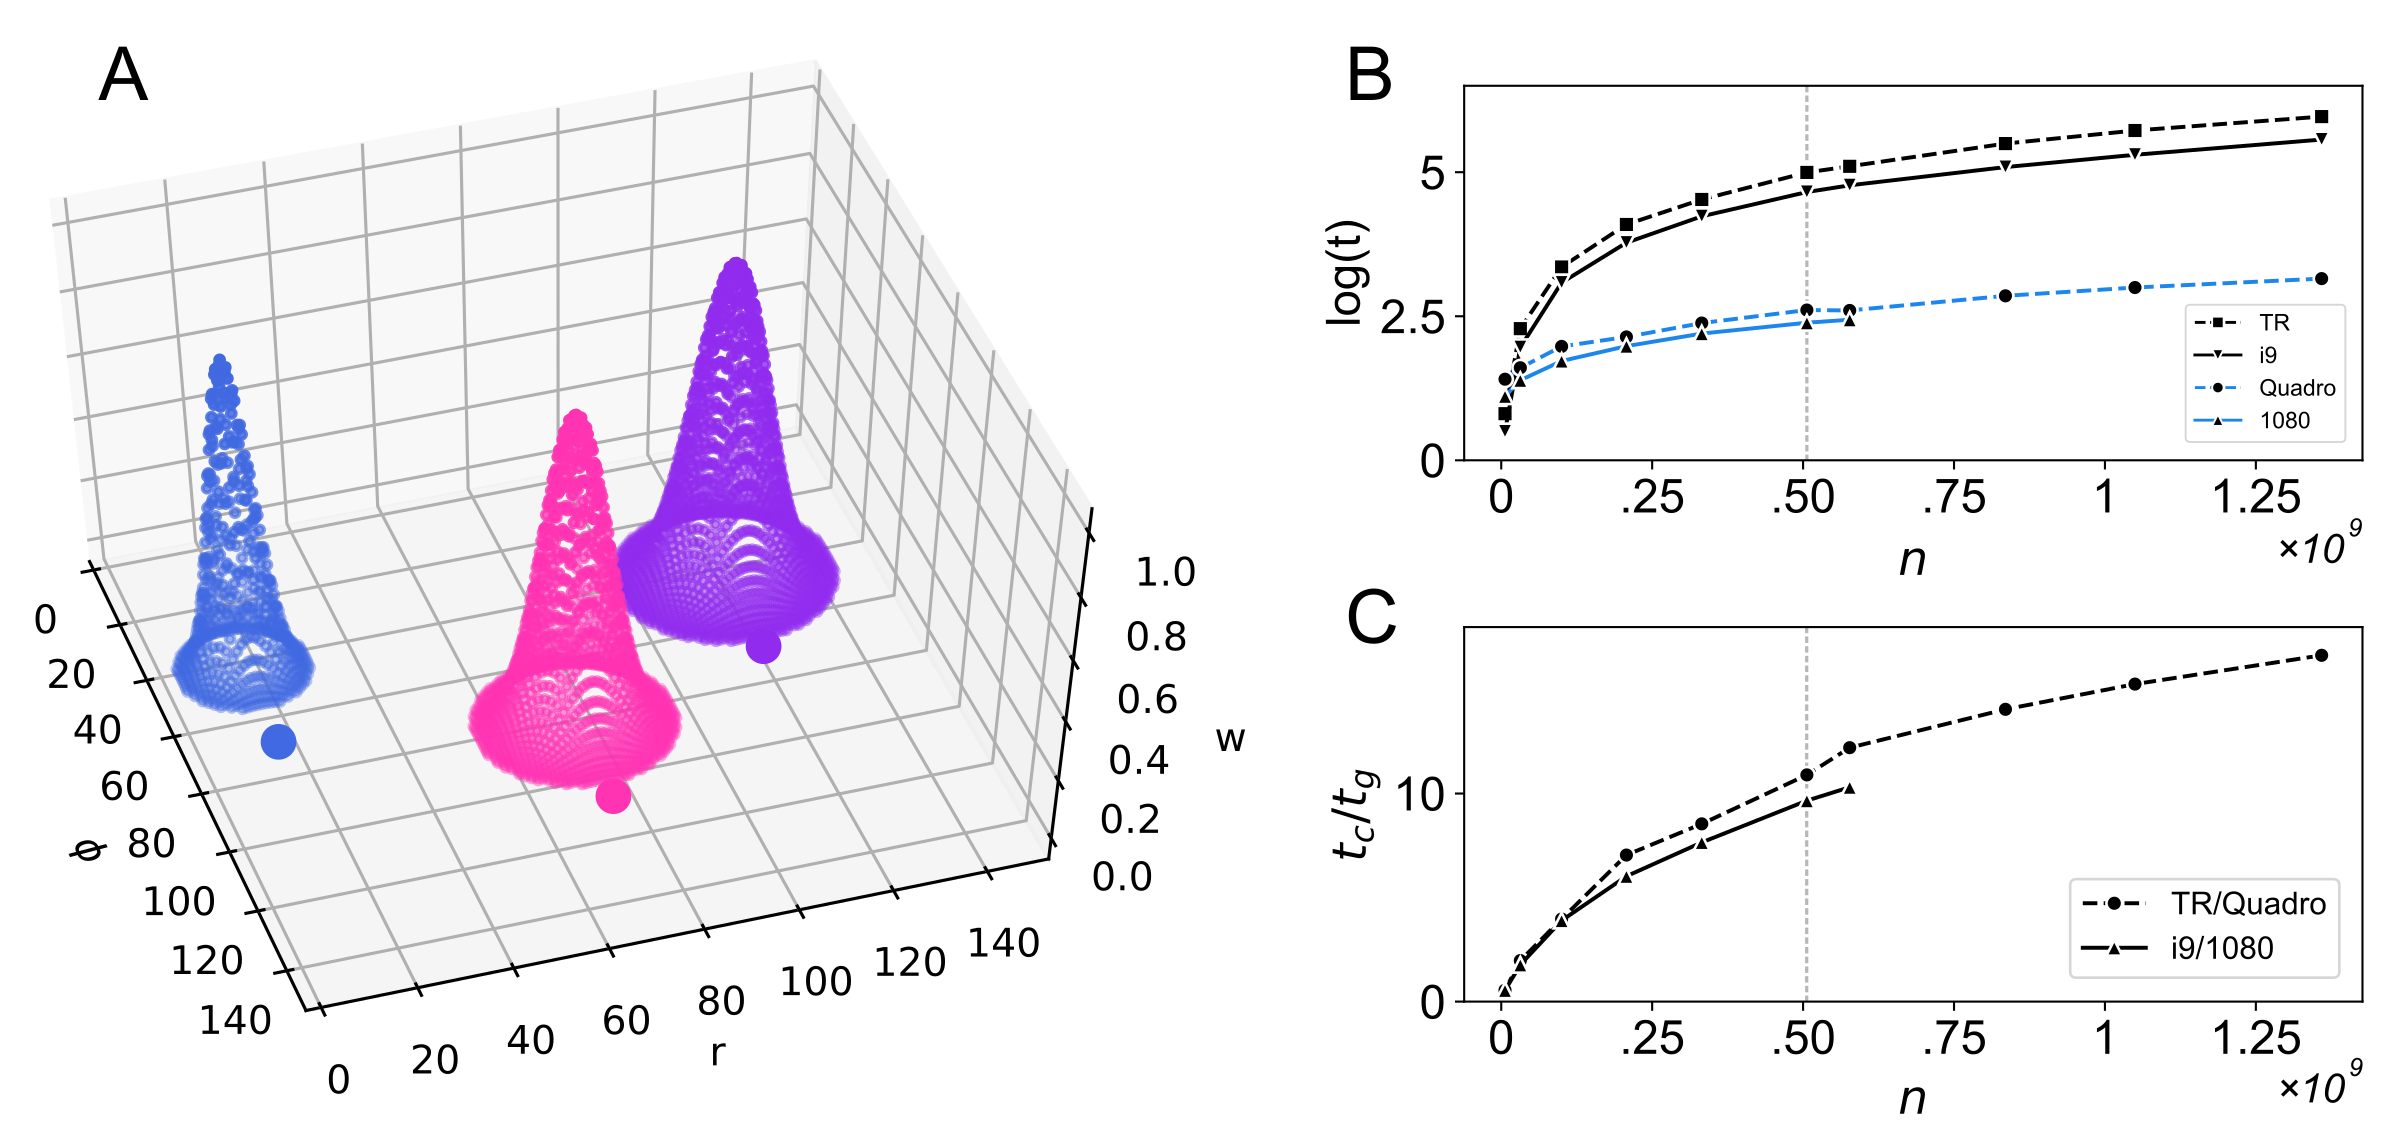
\includegraphics[width=0.95\textwidth]{./fig1.png}
\caption{\textbf{A} Projection patterns computed using the widening gaussian
defined in the appendix code. Projection weights are plotted for three source
neurons, whose locations are shown by large circles. This projection has an
offset in the $\phi$ direction (\code{offsetd0p}) of -25. Other parameters:
\code{sigma\_m}=100, \code{W\_cut}=0.008, \code{fshift}=4, \code{sigma\_0}=3. With
these parameters, a weight table of 22,208,750 rows is generated.
%
\textbf{B}
Log of computation time (in seconds) plotted versus $n$, the maximum possible
number of weights in a projection from a population of size $d^2$ to a second
population of size $d^2$. The dotted grey lines indicate $n$ for the
population size shown in A. Results are shown for an AMD Threadripper 2990WX
CPU (TR), an Intel Core i9-8950HK CPU (i9), an NVIDIA Quadro P5000 GPU and a
GTX 1080 GPU. For small $n$, the overhead in the GPU algorithm makes it slower
than the CPU algorithm. The crossover occurs at $n\approx1.7\times10^6$
($d\approx64$).
%
\textbf{C} Speed-up: The time taken on the CPU ($t_c$) divided by the
time taken on the GPU ($t_g$) plotted vs. $n$ for two different machines (the
Quadro GPU was paired with the Threadripper CPU; the 1080 with the i9). The
overall speed-up exceeds one order of magnitude for populations of the size
shown in A. The data for the i9/1080 is truncated because the 1080 GPU did not
have enough RAM to compute patterns for $d>155$.}
\vspace{-10pt}
\label{f1}
\end{figure}

Execution of the listing in Appendix A takes about 100~s on a fast (Intel i9)
CPU. Although this is not a long wait, the modeller is likely to need to run
the operation many times during model development, to experiment with
different parameters in the connection patterns. The visual attention model
which forms our example has at least 20 different projections, so changing a
common parameter could result in nearly an hour of computation, making the
model exceedingly tedious to work with.  The majority of the time required for
the computation occurs in the inner loop over the destination neurons (line
23). Because each computation in the inner-loop is fully independent, the
computation would seem to be a great candidate for execution on the
GPU. However, at first sight, it appears to be necessary to transfer the
506,250,000 inner-loop results from GPU memory to CPU memory, then carry out
all 506,250,000 weight
\emph{comparisons} in order to sequentially build an ordered, reduced table of
connections, effectively losing any performance gain provided by the GPU!

The solution is to make use of the \emph{parallel prefix scan}
algorithm\cite{blelloch_prefix_1990}. This provides a way of computing the sum
of a set of numbers by summing in blocks and propagating the partial sums
until a final result is produced. Parallel prefix scan can be used to select
out the non-zero weights with a method called \emph{stream
compaction}~\cite{harris_chapter_2010}. This involves summing 1 for each
non-zero weight and using the cumulative sum as the `line address' in the
output table. This way, the output table (which must be preallocated in
memory) can be populated in parallel by the GPU. Appendix B gives an
implementation in Python, using Numba CUDA~\cite{anaconda_inc_numba_2012} to
enable execution on NVIDIA GPU devices. The example follows the work-efficient
parallel scan~\cite{blelloch_prefix_1990} given in~\cite{harris_chapter_2010},
taking into account features of the GPU's shared memory banks to avoid bank
conflicts. The organisation of the code may seem unusual, with all the GPU
kernel functions being defined \emph{within} the outer \code{connectionFunc}
definition. This ensures that
\code{connectionFunc} can be pasted into the Python script window of
SpineCreator. Within \code{connectionFunc}, there are two main code blocks:
i) \code{dowork} which carries out parallel computation of the weights, and is
similar in structure to the code in Appendix A; and
ii) \code{reduce\_nonzero\_gpu}, which carries out the reduction operation,
extracting the non-zero weights into the final output table.

Execution of the code takes about 6 seconds on a GTX 1080 GPU for populations
of 150$\times$150 neural elements.  Computation of the weights
by \code{dowork} takes just 1 millisecond; the reduce
operation, \code{reduce\_nonzero\_gpu}, requires about 5.8 seconds. When
integrated into SpineCreator, this makes the work-flow of modifying projection
parameters feasible. Fig.\,\ref{f1}B shows GPU and CPU times plotted vs. the
problem size, $n$. The graph in Fig.\,\ref{f1}C shows that the GPU speed-up
for larger populations tends towards about 18 times faster than the CPU code.

It is obvious that the GPU implementation code is significantly more complex
than that for the CPU in Appendix A. The implementation consists of roughly
ten times as many lines of code. Appendix A was coded in less than an hour;
Appendix B took weeks of effort. The order of magnitude increase in complexity
is justified by the order of magnitude speed-up achieved by the GPU code.
%
Additionally, much of the GPU solution code is `boilerplate': To change the
form of the projection, perhaps to implement a new Gabor projection in place
of the Gaussian connectivity, only the \code{dowork} function needs to be
re-implemented. Appendix B thus provides to the computational neuroscience
research community a useful template for GPU computation of connection
patterns.
%
%The code in Appendix B uses most of the 8 GB of GPU RAM on the GTX 1080 to
%compute connectivity between two populations each of size 150$\times$150. This
%device can deal with a maximum population size of 157$\times$157 (607,573,201
%weights). A 16 GB GPU was able to process populations of sizes up to
%192$\times$192 (1,358,954,496 weights). In future work, it may be desirable to
%explore ways of reducing the amount of GPU RAM required for the computation in
%order to enable the generation of connection patterns between larger
%populations.

All code discussed in this letter is publicly available
at \url{https://github.com/ABRG-Models/VisualAttention}.

\section*{Acknowledgements}
I'd like to thank Paul Richmond at The University of Sheffield for originally
suggesting the use of the parallel prefix scan algorithm. This work as
supported by a Collaborative Activity Award, Cortical Plasticity Within and
Across Lifetimes, from the James S McDonnell Foundation (grant
220020516).

\selectlanguage{English}
\bibliographystyle{abbrvnotitle}
\bibliography{GPU}

\newpage
\section*{Appendix A: CPU Code}

CPU code defining a widening Gaussian projection with offset. The code listing
here is taken from the VisualAttention
file \code{connectionFuncs/offset\_retgauss.py}. It can be run standalone,
by executing the script \code{connectionFuncs/offset\_retgauss\_run.py}.

\lstinputlisting[language=Python]{../../connectionFuncs/offset_retgauss_forpaper.py}

\newpage
\section*{Appendix B: GPU Code}

Code listing for the widening Gaussian connectivity pattern in Python Numba
code. This is slightly edited version
of \code{connectionFuncs/offset\_retgauss\_gpu.py} from the VisualAttention
repository. Run with \code{connectionFuncs/offset\_retgauss\_gpu\_run.py}.

\lstinputlisting[language=Python]{../../connectionFuncs/offset_retgauss_gpu_forpaper.py}

\end{document}
